\documentclass[10pt,a4paper]{article}
\usepackage[T1]{fontenc}
\usepackage[utf8]{inputenc}
\usepackage{enumitem}
\usepackage{graphicx}
\usepackage{tabularx}
\usepackage{ltablex}
\usepackage{multirow}
\usepackage{helvet}
\usepackage{hhline}
\usepackage{verbatim}
\usepackage[hidelinks]{hyperref}
\usepackage[a4paper,margin=1in]{geometry}
\usepackage{float}
\usepackage[polish]{babel}

\renewcommand\familydefault{\sfdefault}

\begin{document}
\begin{titlepage}
\centering
{\Large Wydział Matematyki i Nauk Informacyjnych Politechniki Warszawskiej \par}
\vspace{1cm}

\includegraphics[width=0.2\textwidth]{Resources/Images/logo.png} \par
\vspace{5cm}
{\LARGE Aplikacja przeznaczona dla osób\\oglądających seriale telewizyjne \par}
\vspace{0.5cm}
{\Large Jacek Dziwulski, Tymon Felski \par}
\vspace{1.5cm}
{\Large \today \par}
\end{titlepage}

\newpage
\tableofcontents

\newpage
\section{Raport}

\subsection{Opis logiki aplikacji}
Stworzona w ramach projektu aplikacja \textbf{TV Tracker} jest narzędziem skierowanym do osób regularnie oglądających seriale telewizyjne. Jej celem jest zarówno umożliwienie śledzenia ulubionych programów, jak i odkrywanie nowych, ponieważ na podstawie polubionych seriali, aplikacja proponuje odbiorcy nowe, podobne do nich.\\[\baselineskip]
Użytkownik może się zalogować przy pomocy konta założonego na portalu \textbf{Facebook} lub swoim kontem \textbf{Google}. Przy pierwszym logowaniu zostanie utworzone konto, które będzie odpowiadać za gromadzenie informacji o serialach użytkownika.\\[\baselineskip]
Ekran główny aplikacji zawiera karty z nadchodzącymi odcinkami polubionych seriali. Pod zdjęciem użytkownik znajdzie krótki opis fabuły, niezdradzający zbyt wielu szczegółów, a także opcje pozwalające na przejście do opisu całego serialu lub wyszukanie zwiastunu odcinka w serwisie \textbf{YouTube}.
\begin{figure}[H]
\centering
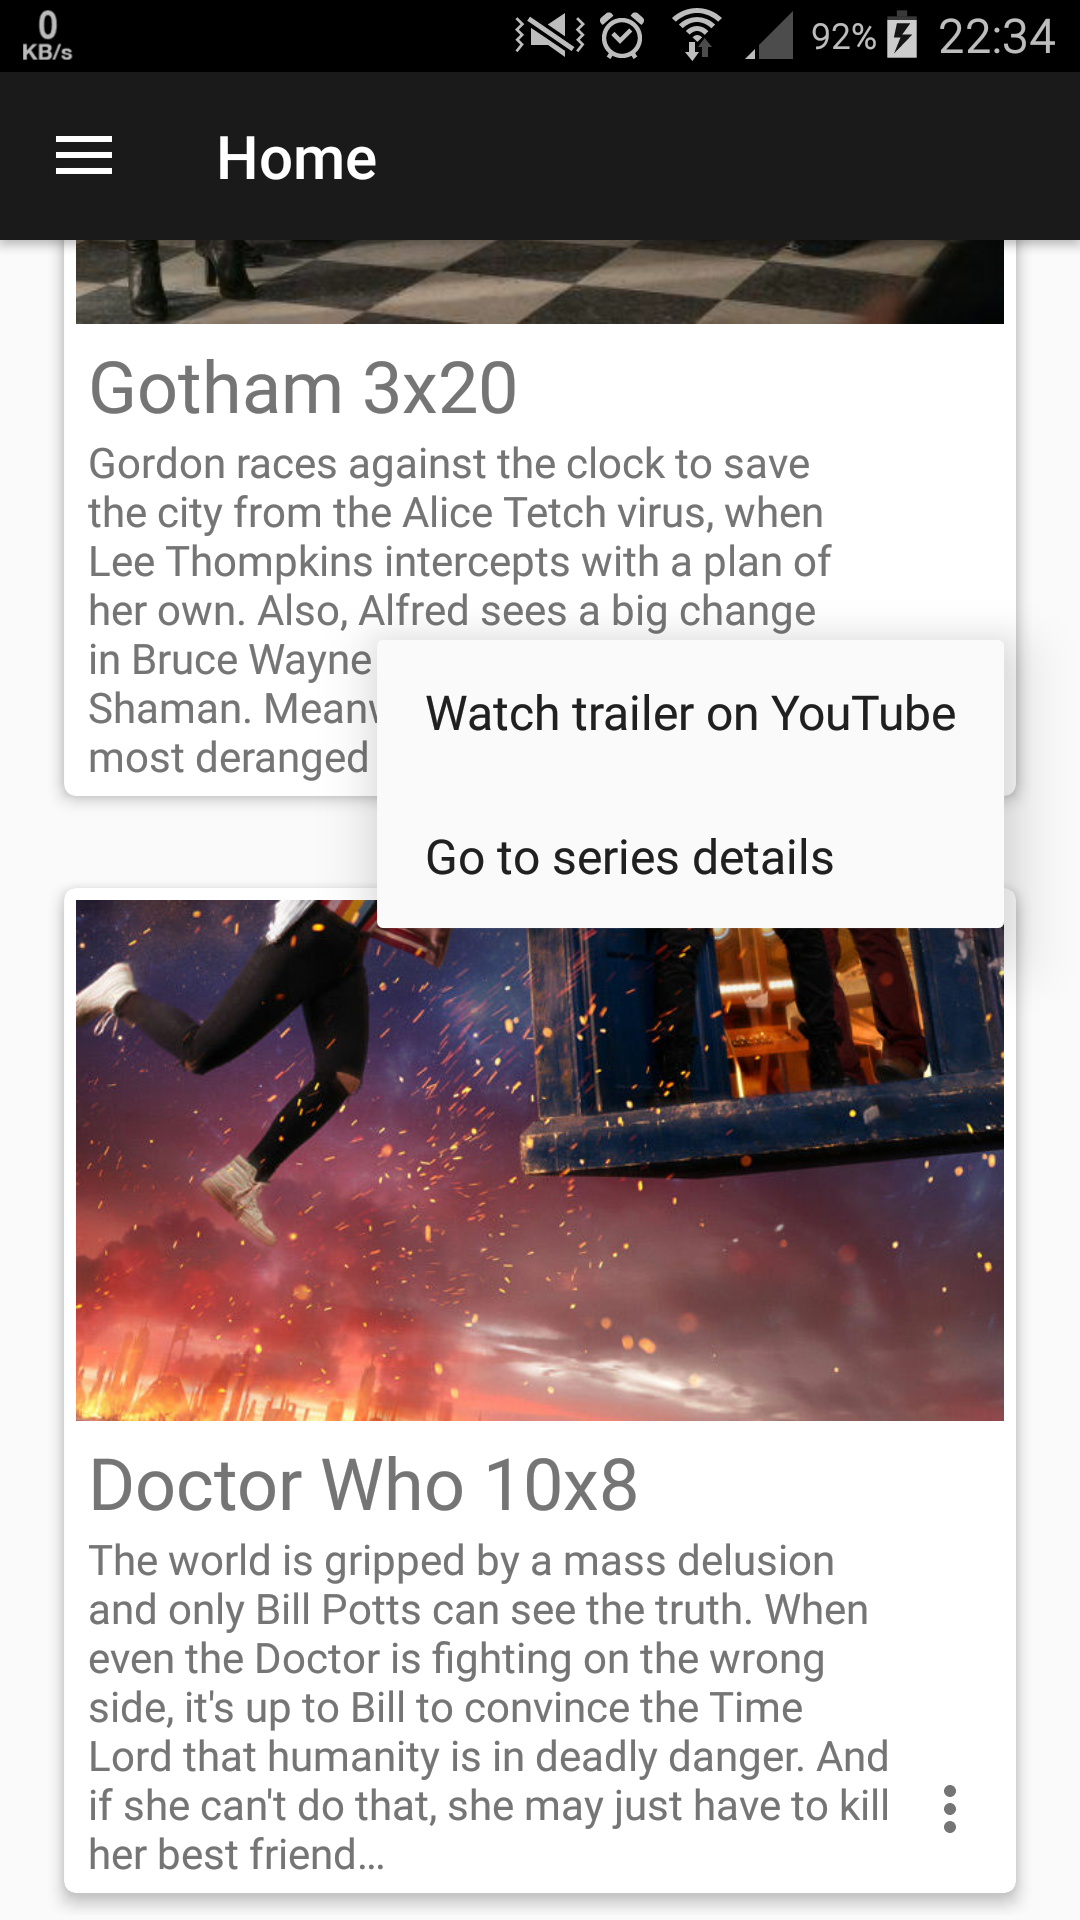
\includegraphics[height=14cm]{Resources/Images/home.png}
\caption{Ekran główny}
\end{figure}
\newpage
\noindent
Nawigacja w aplikacji odbywa się za pomocą panelu bocznego, w którym poza wszystkimi zakładkami znajdzemy także informacje o zalogowanym użytkowniku - jego zdjęcie, imię i nazwisko oraz adres email. Wybranie jednej z zakładek spowoduje zmianę widoku poprzez podmianę fragmentu.
\begin{figure}[H]
\centering
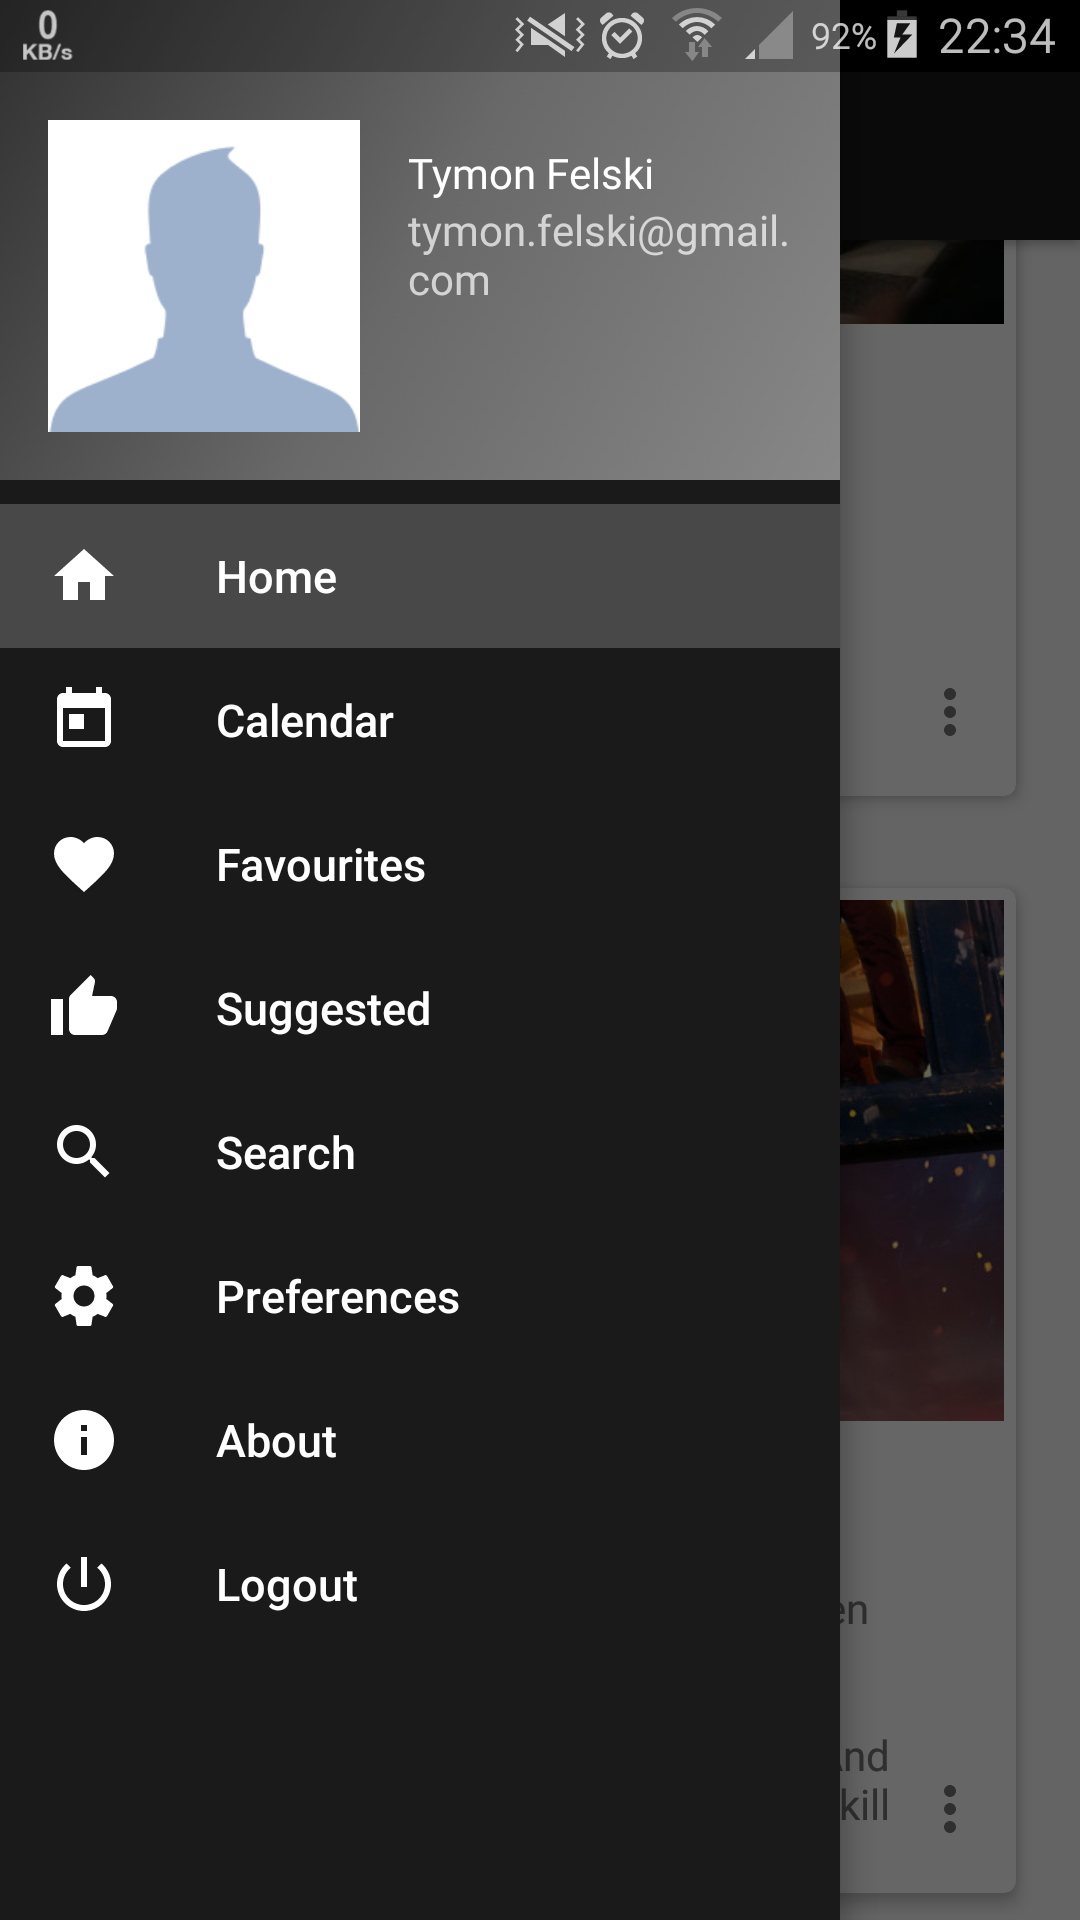
\includegraphics[height=14cm]{Resources/Images/drawer.png}
\caption{Panel boczny}
\end{figure}
\noindent
Aby znaleźć nowe seriale, należy wejść w zakładkę \textbf{Suggested}, w której pojawi się dwadzieścia seriali najlepiej pasujących do obecnie polubionych lub najwyżej oceniane, jeżeli użytkownik nie dodał żadnych do ulubionych. Można także skorzystać z zakładki \textbf{Search}, gdzie po wpisaniu w pole tekstowe przynajmniej trzech znaków pojawią się seriale spełniające kryteria wyszukiwania.\\[\baselineskip]
Ustawienia aplikacji przewidują możliwość ograniczenia transferu danych w jej obrębie poprzez wyłączenie pobierania obrazków lub zastrzeżenie, że mogą być one pobieranie tylko przy pomocy Wi-Fi.
\newpage
\noindent
Zakładka \textbf{Favourites} zawiera polubione przez użytkownika seriale. Można je stąd usunąć lub wejść w dokładny opis jednego z nich, w którym znajdziemy także wszystkie dotychczasowe odcinki. Użytkownik ma możliwość zaznaczania obejrzanych odcinków. Możliwe jest także wyświetlenie dokładnego opisu danego odcinka poprzez kliknięcie w kartę na ekranie głównym lub przytrzymanie nazwy odcinka na wcześniej wspomnianej liście w opisie serialu.
\begin{figure}[H]
\centering
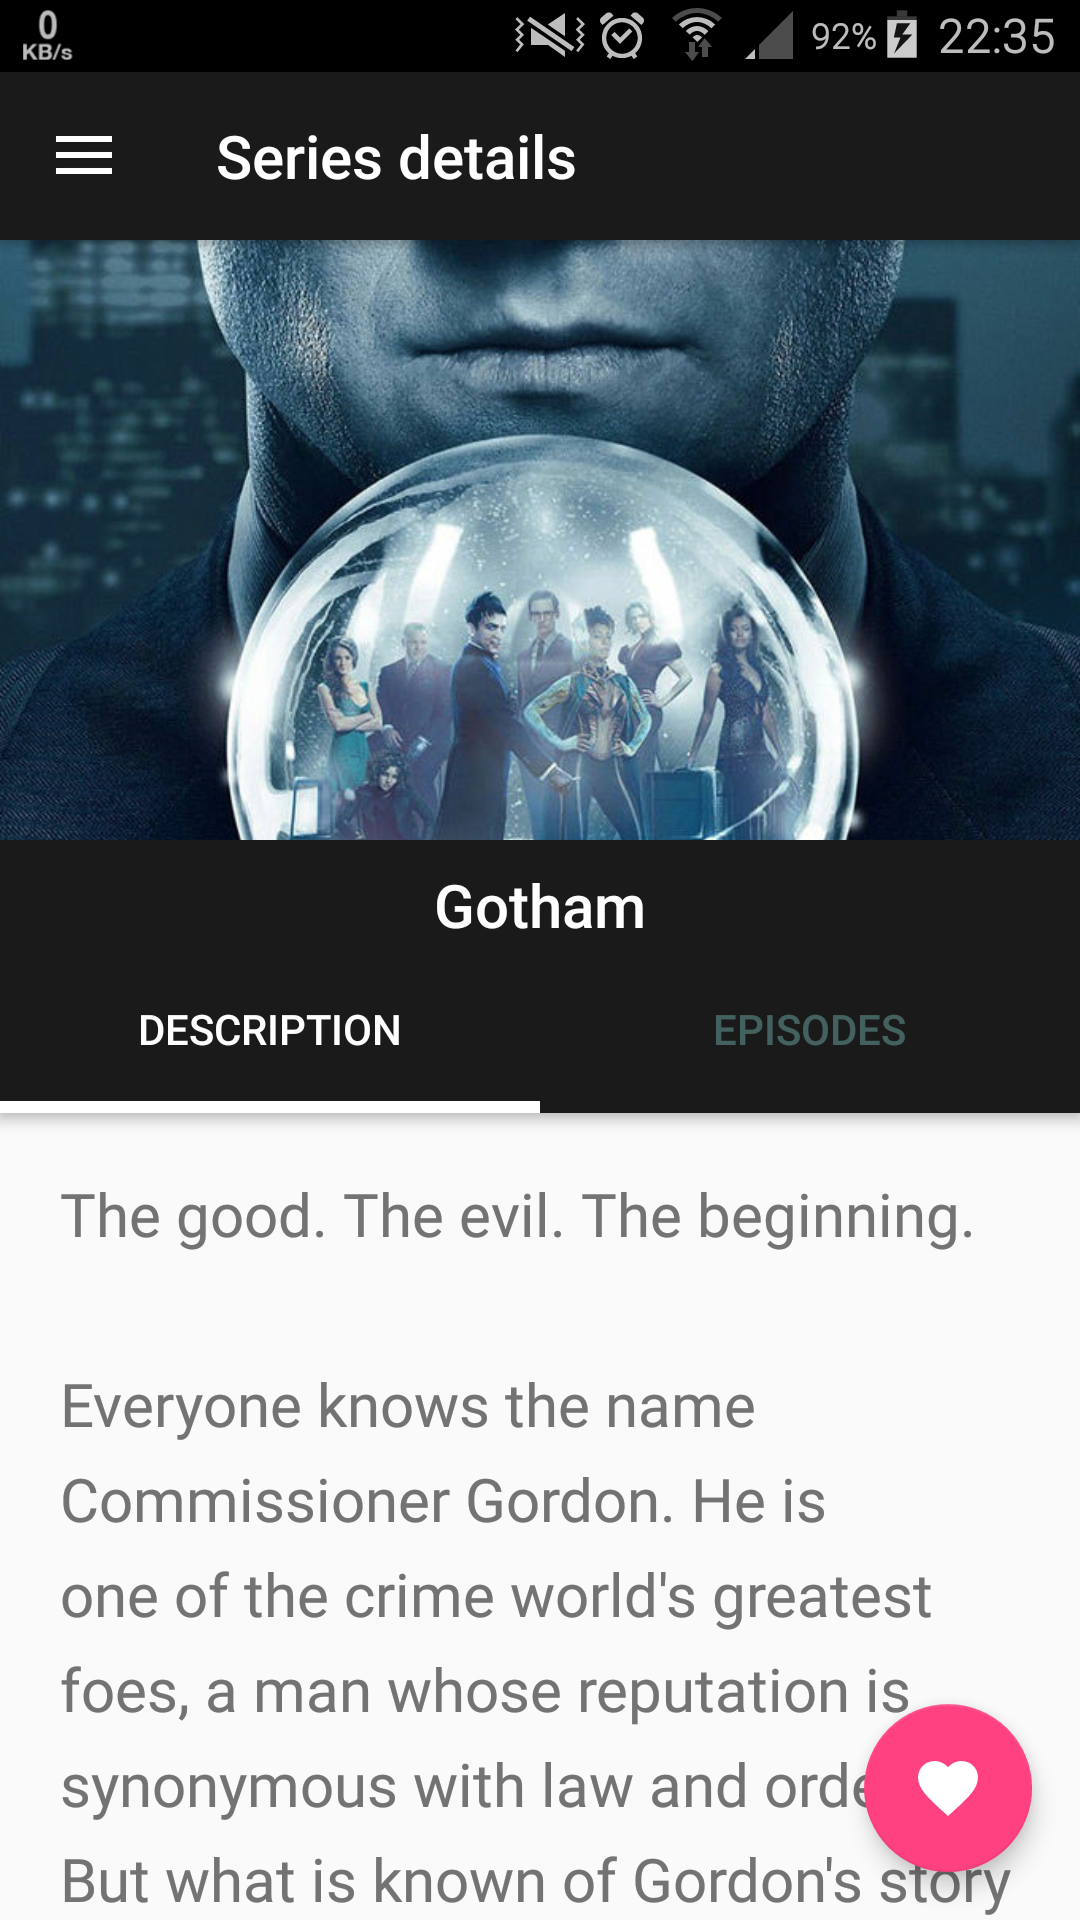
\includegraphics[height=14cm]{Resources/Images/details.png}
\caption{Opis serialu}
\end{figure}
\noindent
W aplikacji znajduje się także kalendarz, w którym można znaleźć wszystkie odcinki z polubionych seriali. Aplikacja wyśle użytkownikowi powiadomienie przypominające o nadchodzącym odcinku nie później niż pół godziny przed jego rozpoczęciem.

\newpage
\subsection{Opis logiki biznesowej}
Wszystkie dane wykorzystywane przez serwer pochodzą z wybranego API, co zostało dokładniej opisane w następnej sekcji. Aby zaoszczędzić czas i transfer danych, pobrane dane zapisywane są we własnej bazie danych. Zapisywane są tam wszystkie informacje o dostępnych programach, a także efekty akcji użytkowników. \\~\\
Użytkownik ma możliwość zalogowania się w aplikacji za pomocą swojego konta Google lub Facebook. Dzięki temu możliwe jest korzystanie z aplikacji na wielu urządzeniach, korzystając z tego samego konta. Zmiany dokonane na jednym urządzeniu, widoczne będą również na pozostałych. W naszej bazie nie przechowujemy szczegółowych informacji o użytkownikach, a jedynie ich identyfikator z wyżej wymienionych serwisów oraz wewnętrzny identyfikator, który jest wymagany, aby można było wykonywać akcje w imieniu użytkownika. \\~\\
Dodatkowo, wykorzystywany jest zewnętrzny serwis - Firebase, udostępniany przez Google. Wykorzystujemy go, aby wysyłać powiadomienia, informujące użytkowników o nadchodzących odcinkach ich ulubionych seriali. Każde urządzenie wykorzystywane przez użytkownika otrzymuje specjalny token identyfikujący to urządzenie. Możliwe jest powiązanie wielu urządzeń z jednym kontem. Dzięki temu użytkownik otrzyma powiadomienia na wszystkich urządzeniach, na których korzysta z naszej aplikacji.

\subsubsection{Wykorzystane API}
Wszystkie dane wykorzystywane przez aplikację pochodzą z publicznego API udostępnianego przez serwis TVmaze \cite{bib8}. Jest to strona zawierająca informacje oraz najnowsze wiadomości dotyczące programów telewizyjnych. Udostępniane API jest darmowe, dostępne na licencji CC BY-SA, co oznacza, że adres do tej strony musi jawnie pojawić się w aplikacji (zakładka \textbf{About}). \\~\\
Liczba zapytań jest limitowana (według zapewnień, możliwe jest wykonanie co najmniej 20 zapytań na 10 sekund, górna granica nie jest ustalona, ale istnieje i zależy od aktualnego obciążenia serwera). Z tego powodu, utworzony przez nas serwer kopiuje wybrane dane do własnej bazy, aby nie było konieczne ciągłe wysyłanie zapytań do API. Raz w tygodniu, przechowywane dane są aktualizowane, aby były zgodne z tymi udostępnianymi przez TVmaze.

\subsubsection{Serwer .NET WebAPI}
Serwer został napisany w technologii .NET, wykorzystując framework ASP.NET WebAPI. Przy uruchomieniu serwera, tworzona jest nowa baza danych, jeśli jeszcze nie istnieje. Następnie, zapisywane są do niej wybrane dane z wykorzystywanego API. Efekty wszystkich operacji wykonywanych przez użytkowników z poziomu aplikacji również są zapisywane w tej bazie. \\~\\
Każdy użytkownik ma przypisany identyfikator, który pozwala mu na modyfikowanie danych powiązanych z jego kontem. Cała komunikacja pomiędzy serwerem a klientem, w której częścią wiadomości jest ten identyfikator, odbywa się przy wykorzystaniu protokołu \textbf{https}, co uniemożliwia uzyskanie identyfikatora użytkownika poprzez podsłuchanie wiadomości.

\newpage
\subsection{Wykorzystane biblioteki wraz z określeniem licencji}
Przy tworzeniu projektu zostały użyte biblioteki zawarte w tabeli poniżej.

\begin{tabularx}{\textwidth}{|r|l|X|l|c|}
\hline
\textbf{Nr} & \textbf{Komponent i wersja} & \textbf{Opis} & \textbf{Licencja} & \\
\hline
\multirow{2}{*}{1} &
\multirow{2}{*}{Android Week View, 1.2.6} &
Kalendarz pozwalający na wyświetlanie wydarzeń &
\multirow{2}{*}{\mbox{\hyperref[abbr:lic]{Apache}}} &
\cite{bib1} \\
\hline
2 &
Floating Search View, 2.0.3 &
Wyszukiwarka wyświetlająca podpowiedzi &
\mbox{\hyperref[abbr:lic]{Apache}} &
\cite{bib2} \\
\hline
\multirow{2}{*}{3} &
\multirow{2}{*}{Butterknife, 8.5.1} &
Biblioteka pozwalająca na bindowanie widoków ze zmiennymi &
\multirow{2}{*}{\mbox{\hyperref[abbr:lic]{Apache}}} &
\cite{bib3} \\
\hline
\multirow{2}{*}{4} &
\multirow{2}{*}{Picasso, 2.5.2} &
Biblioteka pozwalająca na pobieranie, modyfikowanie i przypisywanie do widoków obrazów &
\multirow{2}{*}{\mbox{\hyperref[abbr:lic]{Apache}}} &
\cite{bib4} \\
\hline
\multirow{2}{*}{5} &
\multirow{2}{*}{Retrofit, 2.7} &
Biblioteka pozwalająca na wysyłanie zapytań do API &
\multirow{2}{*}{\mbox{\hyperref[abbr:lic]{Apache}}} &
\cite{bib5} \\
\hline
\multirow{2}{*}{6} &
\multirow{2}{*}{Gson, 2.1.0} &
Biblioteka pozwalająca na konwertowanie reprezentacji JSON na obiekty &
\multirow{2}{*}{\mbox{\hyperref[abbr:lic]{Apache}}} &
\cite{bib6} \\
\hline
7 &
OkHttp, 3.8.0 &
Klient http &
\mbox{\hyperref[abbr:lic]{Apache}} &
\cite{bib7} \\
\hline
\end{tabularx}

\subsection{Wyniki testów z użytkownikami}
Aplikacja została przetestowana przez osoby trzecie. Poniższa tabela zawiera opisy i wyniki tych testów. Wszystkie uwagi zostały rozpatrzone i wprowadziliśmy niezbędne poprawki do aplikacji.

\begin{tabularx}{\textwidth}{|l|X|}
	\hline
	\textbf{Nazwa testu} & Zalogowanie się \\
	\hline
	\textbf{Opis} & Wybranie opcji zalogowania się przy pomocy konta \textbf{Facebook} lub \textbf{Google} \\
	\hline
	\textbf{Oczekiwany wynik} & Przejście do ekranu głównego i pobranie informacji o serialach użytkownika \\
	\hline
	\textbf{Wynik testu} & Pozytywny \\
	\hline
	\textbf{Uwagi} & Brak spinnera sygnalizującego proces logowania \\
	\hhline{==}
	\textbf{Nazwa testu} & Wylogowanie się \\
	\hline
	\textbf{Opis} & Wybranie opcji \textbf{Logout} w bocznym panelu aplikacji \\
	\hline
	\textbf{Oczekiwany wynik} & Przejście do ekranu logowania \\
	\hline
	\textbf{Wynik testu} & Pozytywny \\
	\hline
	\textbf{Uwagi} & Brak \\
	\hhline{==}
	\textbf{Nazwa testu} & Zmiana widoków poprzez wybieranie zakładek w panelu bocznym aplikacji \\
	\hline
	\textbf{Opis} & Wybranie jednej z opcji w bocznym panelu aplikacji \\
	\hline
	\textbf{Oczekiwany wynik} & Przejście do odpowiedniego widoku \\
	\hline
	\textbf{Wynik testu} & Pozytywny \\
	\hline
	\textbf{Uwagi} & Brak \\
	\hhline{==}
	\textbf{Nazwa testu} & Dodanie nowego serialu spośród polecanych \\
	\hline
	\textbf{Opis} & Wybranie jednego z polecanych seriali w zakładce \textbf{Suggested}, przejście do jego szczegółów poprzez kliknięcie i wciśnięcie przycisku dodania do ulubionych \\
	\hline
	\textbf{Oczekiwany wynik} & Dodanie serialu do ulubionych i powiadomienie poprzez snackbar \\
	\hline
	\textbf{Wynik testu} & Pozytywny \\
	\hline
	\textbf{Uwagi} & Brak \\
	\hhline{==}
	\textbf{Nazwa testu} & Dodanie nowego serialu poprzez wyszukanie \\
	\hline
	\textbf{Opis} & Wpisane nazwy serialu w pole tekstowe w zakładce \textbf{Search}, przejście do jego szczegółów poprzez kliknięcie i wciśnięcie przycisku dodania do ulubionych \\
	\hline
	\textbf{Oczekiwany wynik} & Dodanie serialu do ulubionych i powiadomienie poprzez snackbar \\
	\hline
	\textbf{Wynik testu} & Pozytywny \\
	\hline
	\textbf{Uwagi} & Brak \\
	\hhline{==}
	\textbf{Nazwa testu} & Usunięcie serialu z ulubionych \\
	\hline
	\textbf{Opis} & Przesunięcie wybranego serialu w lewo lub w prawo w zakładce \textbf{Favourites} \\
	\hline
	\textbf{Oczekiwany wynik} & Usunięcie serialu z ulubionych i powiadomienie poprzez snackbar \\
	\hline
	\textbf{Wynik testu} & Pozytywny \\
	\hline
	\textbf{Uwagi} & Brak możliwości cofnięcia usunięcia \\
	\hline
	\textbf{Nazwa testu} & Cofnięcie usunięcia serialu z ulubionych \\
	\hline
	\textbf{Opis} & Usunięcie serialu/serialów z ulubionych i wciśnięcie przycisku \textbf{UNDO} na snackbarze \\
	\hline
	\textbf{Oczekiwany wynik} & Przywrócenie serialu/serialów do ulubionych i powiadomienie poprzez snackbar \\
	\hline
	\textbf{Wynik testu} & Pozytywny \\
	\hline
	\textbf{Uwagi} & Brak \\
	\hhline{==}
	\textbf{Nazwa testu} & Zmiana ustawień pobierania obrazków \\
	\hline
	\textbf{Opis} & W zakładce \textbf{Preferences} wybranie jednej z opcji pobierania obrazków \\
	\hline
	\textbf{Oczekiwany wynik} & Całkowite wyłączenie pobierania obrazków lub ograniczenie do Wi-Fi \\
	\hline
	\textbf{Wynik testu} & Pozytywny \\
	\hline
	\textbf{Uwagi} & Brak \\
	\hline
\end{tabularx}

\section{Lista użytych skrótów}
\label{abbr:lic}
\paragraph{Apache} Apache License Version 2.0, \url{http://www.apache.org/licenses/LICENSE-2.0}

\renewcommand*{\refname}{\vspace*{-2em}}
\section{Bibliografia}
\begin{thebibliography}{99}

\bibitem{bib1}
Android Week View,
\emph{Raquib-ul-Alam},
\url{https://github.com/alamkanak/Android-Week-View}

\bibitem{bib2}
Floating Search View,
\emph{Ari C.},
\url{https://github.com/arimorty/floatingsearchview}

\bibitem{bib3}
Butterknife,
\emph{Jake Wharton},
\url{http://jakewharton.github.io/butterknife/}

\bibitem{bib4}
Picasso,
\emph{Square, Inc.},
\url{http://square.github.io/picasso/}

\bibitem{bib5}
Retrofit,
\emph{Square, Inc.},
\url{http://square.github.io/retrofit/}

\bibitem{bib6}
Gson,
\emph{Google Inc.},
\url{https://github.com/google/gson}

\bibitem{bib7}
OkHttp,
\emph{Square, Inc.},
\url{http://square.github.io/okhttp/}

\bibitem{bib8}
TVmaze,
\url{http://www.tvmaze.com/}

\end{thebibliography}

\end{document}